\documentclass[12pt]{article}
\usepackage{epsfig}
\usepackage{url}
\usepackage{verbatim}
\usepackage{amsmath}
\usepackage{amsfonts}

\newcommand{\wc}[1]{\textit{todo: #1}}
\newcommand{\ct}[1]{\textit{cite: #1}}
\newcommand{\cd}[1]{\texttt{#1}}
\newcommand{\trm}[1]{\textit{#1}}
\newcommand{\vek}[1]{\textbf{#1}}

\newcommand{\loss}{\textit{L}}
\newcommand{\deriv}[2]{\frac{d{}#1}{d{}#2}}

\title{Automatic Reverse-Mode Differentiation}

\author{William Cohen\\ Modified by xxx}
\date{Out xxx\\Due xxx via Blackboard}

\begin{document}

\maketitle

\section{Background: Automatic Differentiation}

\subsection{Why automatic differentiation is important}

Most neural network packages (e.g., Torch or Theano) don't require a
user to actually derive the gradient updates for a neural model.
Instead they allow the user to define a \trm{model} in a ``little
language'', which supports common neural-network operations like
matrix multiplication, ``soft max'', etc, and automatically derive the
gradients.  Typically, the user will define a \trm{loss function}
$\loss$ in this sublanguage: the loss function takes as inputs the
training data, current parameter values, and hyperparameters, and
outputs a scalar value. From the definition of $\loss$, the system
will compute the partial derivative of the loss function with respect
to every parameter, using these gradients, it's straightforward bto
implement gradient-based learning methods.

Going from the definition of $\loss$ to its partial derivatives is
called \trm{automatic differentiation}.  In this assignment you will
start with a simple automatic differentiation system written in
Python, and use it to implement a neural-network package.

\subsection{Wengert lists}

Automatic differentiation proceeds in two stages.  First, function
definitions $f(x_1,\ldots,x_k)$ in the sublanguage are converted to a
format called a \trm{Wengert list}.  The second stage is to evaluate
the function and its gradients using the Wengert list.

A \trm{Wengert list} defines a function $f(x_1,\ldots,x_k)$ of some
inputs $x_1,\ldots,x_k$.  Syntactically, it is just a list of
assignment statements, where the right-hand-side (RHS) of each
statement is very simple: a call to a function $g$ (where $g$ is one
of a set of primitive functions $G=\{g_1,\ldots,g_\ell\}$ supported by
the sublanguage), where the arguments to $g$ either inputs
$x_1,\ldots,x_k$, or the left-hand-side (LHS) of a previous
assignment.  (The functions in $G$ will be called \trm{operators}
here.)  The output of the function is the LHS of the last item in the
list.  For example, a Wengert list for
\begin{equation} \label{eq:2x1Plusx2}
f(x_1,x_2) \equiv (2 x_1 + x_2)^2
\end{equation} 
with the functions $G = \{ \cd{add},\cd{multiply},\cd{square} \}$ might be
\begin{eqnarray*}
z_1 & = & \cd{add}(x_1,x_1) \\
z_2 & = & \cd{add}(z_1,x_2) \\
f & = & \cd{square}(z_2)
\end{eqnarray*}
A Wengert list for
\[ f(x) \equiv x^3
\] 
might be
\begin{eqnarray*}
z_1 & = & \cd{multiply}(x,x) \\
f & = & \cd{multiply}(z_1,x)
\end{eqnarray*}

The set of functions $G$ defines the sublanguage.  It's convenient if
they have a small fixed number of arguments, and are differentiable
with respect to all their arguments.  But there's no reason that they
have to be scalar functions!  For instance, if $G$ contains the
appropriate matrix and vector operations, the loss for logistic
regression (for example $\vek{x}$ with label $y$ and weight matrix
$W$) could be written as
\[ f(\vek{x},\vek{y},W) \equiv 
      \cd{crossEntropy}( \cd{softmax}(\vek{x} \cdot W ), \vek{y}) + \cd{frobeniusNorm}(W)
\] 
and be compiled to the Wengert list
\begin{eqnarray*}
 \vek{z}_1 & = & \cd{dot}(\vek{x},W) \\
 \vek{z}_2 & = & \cd{softmax}(\vek{z}_1) \\
 z_3 & = & \cd{crossEntropy}(\vek{z}_2,\vek{y}) \\
 z_4 & = & \cd{frobeniusNorm}(W) \\
 f & = & \cd{add}(z_3,z_4)
\end{eqnarray*}
This implements $k$-class logistic regression if $\vek{x}$ is a
$d$-dimensional row vector, \cd{dot} is matrix product, $W$ is a $d
\times k$ weight matrix, and 
\begin{eqnarray*}
 \cd{softmax}(\langle a_1,\ldots,a_d\rangle) & \equiv &
   \langle \frac{e^{a_1}}{\sum_{i=1}^d e^a_i}, \ldots, \frac{e^{a_d}}{\sum_{i=1}^d e^a_i} \rangle  \\
 \cd{crossEntropy}(\langle a_1,\ldots,a_d\rangle,\langle b_1,\ldots,b_d\rangle) & \equiv &
    - \sum_{i=1}^d a_i \log b_i \\
 \cd{frobeniusNorm}(A) & \equiv & \sqrt{ \sum_{i=1}^d \sum_{j=1}^k a_{i,j}^2 }
\end{eqnarray*}

\subsection{Backpropagation through Wengert list}

We'll first discuss how to use a Wengert list, and then below, discuss
how to construct one.

Given a Wengert list for $f$, it's obvious how to evaluate $f$: just
step through the assignment statements in order, computing each value
as needed.  To be perfectly clear about this, the procedure is as
follows.  We will encode each assignment in Python as a nested tuple
\[ (z, g, (y_1,\ldots,y_k))
\]
where $z$ is a string that names the LHS variable, $g$ is a string
that names the operator, and the $y_i$'s are strings that name the
arguments to $g$.  So the list for the function of
Equation~\ref{eq:2x1Plusx2} would be encoded in python as
\begin{verbatim}
[ ("z1", "add", ("x1","x2")), 
  ("z2", "add", ("z1","x2")), 
  ("f", "square", ("z2")) ]
\end{verbatim}
We also store functions for each operator in a Python dictionary
\cd{G}:
\begin{verbatim}
G = { "add" : lambda a,b: a+b, 
       "square": lambda a:a*a }
\end{verbatim}
Before we evaluate the function, we will store the parameters in a
dictionary \cd{val}: e.g., to evalute $f$ and $x_1=3$, $x_2=7$
we will initialize \cd{val} to 
\begin{verbatim}
val = { "x1" : 3, "x2" : 7 }
\end{verbatim}

The pseudo-code to evaluate $f$ is:

\begin{tabbing}1234\=1234\=\kill
\cd{def eval($f$)} \\
\> initialize \cd{val} to the inputs at which $f$ should be evaluated\\
\> \cd{for} $(z,g,(y_1,\ldots,y_k))$ in the list:\\
\>     \> \cd{op = G[g]} \\
\>     \> \cd{val[z] = op(val[$y_1$],\ldots,val[$y_k$])}\\
\> \cd{return} the last entry stored in \cd{val}.
\end{tabbing}

\textit{Some Python hints:} (1) to convert $(y_1,\ldots,y_k)$ to
\cd{(val[$y_1$],\ldots,val[$y_k$])} you might use Python's \cd{map}
function. (2) If \cd{args} is a length-2 Python list and \cd{g} is a
function that takes two arguments (like \cd{G[``add'']} above) then
\cd{g(*args)} will call \cd{g} with the elements of that list as the
two arguments to \cd{g}.

To differentiate, we will use a generalization of backpropagation
(backprop). We'll assume that \cd{eval} has already been run and
\cd{val} has been populated, and we will compute, in \emph{reverse}
order, a value \cd{delta}($z_i$) for each variable $z_i$ that appears
in the list.  We initialize \cd{delta} by setting $\cd{delta}(f)=1$,
(where $f$ is the string that names the function output).  

Informally you can think of \cd{delta}($z_i$) as the ``sensitivity''
of $f$ to the variable $z_i$, , at the point we're evaluating $f$
(i.e., the point $a$ that corresponds to the initial dictionary
entries we stored in \cd{val}). Here $z_i$ can be intermediate
variable or an input.  If it's an input $x$ that we're treating as a
parameter, \cd{delta} is the gradient of the cost function, evaluated
at $a$: i.e., $\cd{delta}(x) = \deriv{f}{x}(a)$.  

To compute these sensitivities we need to ``backpropagate'' through
the list: when we encounter the assignment \((z,g,(y_1,\ldots,y_k))\)
we will use \cd{delta}($z$) and the derivatives of $g$ with respect to
its inputs to compute the sensitivities of the $y$'s.  We will store
derivatives for each operator in a Python dictionary \cd{DG}. 

Note that if $g$ has $k$ inputs, then we need $k$ partial derivatives,
one for each input, so the entries in \cd{DG} are \emph{lists} of
functions. For the functions used in this example, we'll need
these entries in DG.
\begin{verbatim}
DG = { "add" : [ (lambda a,b: 1),  (lambda a,b: 1) ],  
       "square": [ lambda a:2*a ] }
\end{verbatim}
To figure out these functions we used some high school calculus rules:
$\deriv{}{x}(x+y)=1$, $\deriv{}{y}(x+y)=1$ and $\deriv{}{x}(x^2)=2x$.

Finally, the pseudo-code to compute the deltas is below.  Note that we
don't just store values in \cd{delta}: we accumulate them additively.

\begin{tabbing}1234\=1234\=1234\=1234\=\kill
\cd{def backprop($f$,val)} \\
\> initialize \cd{delta}: \cd{delta}[$f$] = 1\\
\> \cd{for} \cd{(z,g,($y_1,\ldots,y_k$))} in the list, in reverse order:\\
\>     \> \cd{for} $i=1,\ldots,k$:\\
\>     \>    \> \cd{op$_i$ = DG[g][$i$]} \\
\>     \>    \> \cd{if delta[$y_i$]} is not defined set \cd{delta[$y_i$] = 0} \\
\>     \>    \> \cd{delta}[$y_i$] = \cd{delta}[$y_i$] + \cd{delta[z] * op$_i$(val[$y_1$],\ldots,val[$y_k$])}\\
\end{tabbing}

\subsection{Examples}

Let's look at Equation~\ref{eq:2x1Plusx2}.  In freshman calculus
you'd just probably just do this: 
\begin{eqnarray*}
f(x_1,x_2) & = & (2 x_1 + x_2)^2 = 4 x_1^2 + 4 x_1 x_2 + x_2^2 \\
\deriv{f}{x_1} & = & 8 x_1 + 4 x_2 \\
\deriv{f}{x_2} & = & 4 x_1 + 2 x_2 \\
\end{eqnarray*}

\begin{table}
\begin{tabular}{l|l}
Derivation Step & Reason \\
\hline
\( \deriv{f}{x_1}  =  \deriv{z_2^2}{z_2} \cdot \deriv{z_2}{x_1} \)
         & $f=z_2^2$ \\
& \\
\( \deriv{f}{x_1}  =  2 z_2 \cdot \deriv{z_2}{x_1} \)
         & $\deriv{(a^2)}{a} = 2a$ \\
& \\
\( \deriv{f}{x_1}  =  2 z_2 \cdot \deriv{(z_1 + x_2)}{x_1} \)
         & $z_2 = z_1 + x_2$ \\
& \\
\( \deriv{f}{x_1}  =  2 z_2 \cdot \left( 1 \cdot \deriv{z_1}{x_1} + 1 \cdot \deriv{x_2}{x_1} \right) \)
         & $\deriv{(a+b)}{a} = \deriv{(a+b)}{b} = 1$ \\
& \\
\( \deriv{f}{x_1}  =  2 z_2 \cdot \left( 1 \cdot \deriv{(x_1 + x_1)}{x_1} + 1 \cdot \deriv{x_2}{x_1} \right) \)
         & $z_1 = x_1 + x_1$ \\
& \\
\( \deriv{f}{x_1}  =  2 z_2 \cdot \left( 1 \cdot \left( 1 \cdot \deriv{x_1}{x_1} + 1 \cdot \deriv{x_1}{x_1} \right) + 1 \cdot \deriv{x_2}{x_1} \right) \)
         & $\deriv{(a+b)}{a} = \deriv{(a+b)}{b} = 1$ \\
& \\
\( \deriv{f}{x_1}  =  2 z_2 \cdot \left( 1 \cdot \left( 1 \cdot 1 + 1 \cdot 1 \right) + 1 \cdot 0 \right) \)
         & $\deriv{a}{a}=1$ and $\deriv{a}{b}=0$ for inputs $a,b$ \\
& \\
\( \deriv{f}{x_1}  =  2 z_2 \cdot 2 = 8 x_1 + 4 x_2 \) 
         & simplify\\
\hline
\end{tabular}
\caption{A detailed derivation of $\deriv{f}{x_1}$ for $f = z_2^2; z_2 = z_1 + x_2; z_1 = x_1 + x_1$}
\label{dx1:2x1Plusx2}
\end{table}

Here we'll use the Wengert list, in reverse, and the chain rule.  This
list is
\begin{eqnarray*}
z_1 & = & \cd{add}(x_1,x_1) \\
z_2 & = & \cd{add}(z_1,x_2) \\
f & = & \cd{square}(z_2)
\end{eqnarray*}
Table~\ref{dx1:2x1Plusx2} contains a detailed derivation of
$\deriv{f}{x_1}$, where in each step we either plug in a definition of
a variable in the list, or use the derivative of one of the operators
(\cd{square} or \cd{add}). Table~\ref{dx2:2x1Plusx2} contains an
analogous derivation of $\deriv{f}{x_1}$.  Notice that these
derivations are nearly identical.  In fact, they are very analogous to
the computations carried out by the \cd{backprop} algorithm: can you
see how?

\begin{table}
\begin{tabular}{l|l}
Derivation Step & Reason \\
\hline
\( \deriv{f}{x_2}  =  \deriv{z_2^2}{z_2} \cdot \deriv{z_2}{x_2} \)
         & $f=z_2^2$ \\
& \\
\( \deriv{f}{x_2}  =  2 z_2 \cdot \deriv{z_2}{x_2} \)
         & $\deriv{(a^2)}{a} = 2a$ \\
& \\
\( \deriv{f}{x_2}  =  2 z_2 \cdot \deriv{(z_1 + x_2)}{x_2} \)
         & $z_2 = z_1 + x_2$ \\
& \\
\( \deriv{f}{x_2}  =  2 z_2 \cdot \left( 1 \cdot \deriv{z_1}{x_2} + 1 \cdot \deriv{x_2}{x_2} \right) \)
         & $\deriv{(a+b)}{a} = \deriv{(a+b)}{b} = 1$ \\
& \\
\( \deriv{f}{x_2}  =  2 z_2 \cdot \left( 1 \cdot \deriv{(x_1 + x_1)}{x_2} + 1 \cdot \deriv{x_2}{x_2} \right) \)
         & $z_1 = x_1 + x_1$ \\
& \\
\( \deriv{f}{x_2}  =  2 z_2 \cdot \left( 1 \cdot \left( 1 \cdot \deriv{x_2}{x_2} + 1 \cdot \deriv{x_1}{x_2} \right) + 1 \cdot \deriv{x_2}{x_2} \right) \)
         & $\deriv{(a+b)}{a} = \deriv{(a+b)}{b} = 1$ \\
& \\
\( \deriv{f}{x_1}  =  2 z_2 \cdot \left( 1 \cdot \left( 1 \cdot 1 + 1 \cdot 0 \right) + 1 \cdot 1 \right) \)
         & $\deriv{a}{a}=1$ and $\deriv{a}{b}=0$ for inputs $a,b$ \\
& \\
\( \deriv{f}{x_1}  =  2 z_2 \cdot 2 = 4 x_1 + 2 x_2 \) 
         & simplify\\
\hline
\end{tabular}
\caption{A detailed derivation of $\deriv{f}{x_2}$ for $f = z_2^2; z_2 = z_1 + x_2; z_1 = x_1 + x_1$}
\label{dx2:2x1Plusx2}
\end{table}

\begin{table}
\begin{tabular}{l|l}
Derivation Step & Reason \\
\hline
\( \deriv{f}{x}  =  \deriv{z_1}{x} x  +  z_1 \deriv{x}{x} \)
         & $f=z_1 x$ and $\deriv{(ab)}{x} = \deriv{a}{x}b + a\deriv{b}{x}$ \\
& \\
\( \deriv{f}{x_1}  =  \left( \deriv{x}{x} x + x \deriv{x}{x} \right)  \cdot x +  z_1 \deriv{x}{x} \)
         & $z_1 = x\cdot x$ and $\deriv{(ab)}{x} = \deriv{a}{x}b + a\deriv{b}{x}$ \\
& \\
\( \deriv{f}{x_1}  =  \left( x + x \right)  \cdot x +  x^2  = 3 x^2 \)
         & $z_1 = x\cdot x$ and simplify \\
\hline
\end{tabular}
\caption{A derivation of $\deriv{f}{x}$ for $f = z_1; z_1 = x x$ }
\label{dx:xcubed}
\end{table}

Finally Table~\ref{dx:xcubed} shows a slightly less detailed
derivation of the second sample function, $f = x^3$.  It is
instructive to step through the \cd{backprop} algorithm for these
functions as well: for example the list $z_1 = x\cdot x; f = z_1 \cdot x$ 
leads to the \cd{delta} updates. 


\begin{eqnarray*}
\cd{delta}[f]   & =  1  \\
\cd{delta}[z_1] & +=  \cd{delta}[f] \cdot x = x & \mbox{arg 1 of $f=$\cd{mul(...)}}\\
\cd{delta}[x]   & +=  \cd{delta}[f] \cdot z_1 = x^2 & \mbox{arg 2 of $f=$\cd{mul(...)}}\\
\cd{delta}[x]   & +=  \cd{delta}[z_1] \cdot x = x^2 & \mbox{arg 1 of $z_1=$\cd{mul(...)}}\\
\cd{delta}[x]   & +=  \cd{delta}[z_1] \cdot x = x^2 & \mbox{arg 1 of $z_1=$\cd{mul(...)}}
\end{eqnarray*}

\subsection{Discussion}

What's going on here? Let's simplify for a minute and assume that the
list is of the form
\begin{eqnarray*}
 z_1 & = &  f_1(z_0) \\
 z_2 & = &  f_2(z_1) \\
 & \ldots & \\
 z_m & = &  f_m(z_{m-1})
\end{eqnarray*}
so $f = z_m = f_m(f_{m-1}(\ldots f_1(z_0) \ldots))$.  We'll assume we
can compute the $f_i$ functions and their derivations $f'_i$.  We know
that one way to find $\deriv{z_m}{z_0}$ would be to repeatedly use the
chain rule:
\begin{eqnarray*}
\deriv{z_m}{z_0} & = & \deriv{z_m}{z_{m-1}} \deriv{z_{m-1}}{z_0} \\
                 & = & \deriv{z_m}{z_{m-1}} \deriv{z_{m-1}}{z_{m-2}} \deriv{z_{m-2}}{z_{0}} \\
 \ldots \\
                 & = &  \deriv{z_m}{z_{m-1}} \deriv{z_{m-1}}{z_{m-2}} \ldots \deriv{z_{1}}{z_{0}}
\end{eqnarray*}
Let's take some time to unpack what this means.  When we do
derivations by hand, we are working symbolically: we are constructing
a \emph{symbolic representation} of the derivative function.  This is
an interesting problem---it's called \trm{symbolic
  differentiation}---but it's not the same task as automatic
differentiation.  In automatic differentiation, we want instead an
\emph{algorithm} for \emph{evaluating} the derivative function.

To simplify notation, let $h_{i,j}$ be the function
$\deriv{z_i}{z_j}$.  (I'm doing this so that I can use $h_{i,j}(a)$ to
denote the result of evaluating the function $\deriv{z_i}{z_j}$ at a:
$\deriv{z_i}{z_j}(a)$ is hard to read.)  Notice that there are $m^2$
of these $h_{i,j}$ functions---quite a few!---but for machine learing
applications we won't care about most of them: typically we just care
about the partial derivative of the cost function (the final variable
in the list) with respect to the parameters, so we only need $h_{m,i}$
for certain $i$'s.

Let's look at evaluating $h_{m,0}$ as some point $z_0=a$ (say
$z_0=53.4$). Again to simplify, define
\begin{eqnarray*}
a_1 & = & f_1(a) \\
a_2 & = & f_2(f_1(a)) \\
 & \ldots & \\
a_m & = & f_{m}(f_{m-1}(f_{m-2}(\ldots f_1(a) \ldots)))
\end{eqnarray*}
When we write
\[
\deriv{z_m}{z_0}  =  \deriv{z_m}{z_{m-1}} \deriv{z_{m-1}}{z_0}
\]
We mean that: for all $a$
\[
h_{m,0}(a) = f'_{m}(a_m) \cdot h_{m-1,1}(a)
\]
That's a useful step because we have assumed we have available a
routine to evaluate $f'_{m}(a_m)$: in the code this would be the
function \cd{DG[$f_m$][1]}.  Continuing, when we write
\begin{eqnarray*}
\deriv{z_m}{z_0} & = & \deriv{z_m}{z_{m-1}} \deriv{z_{m-1}}{z_{m-2}} \ldots \deriv{z_{1}}{z_{0}}
\end{eqnarray*}
it means that 
\[
h_{m,0}(a) = f'_{m}(a_m) \cdot f'_{m-1}(a_{m-1})\cdots f'_{2}(a_1) \cdot f'_{1}(a)
\]
When we execute the \cd{backprop} code above, this is what we do: in particular we
group the operations as 
\[
h_{m,0}(a) = \left(\left(\left( (f'_{m}(a_m) \cdot f'_{m-1}(a_{m-1}) \right) \cdot f'_{m-2}(a_{m-2})\right) \cdots f'_{2}(a_1)) \right) \cdot f'_{1}(a)
\]
and the \cd{delta}'s
are partial products: specifically 
\[ \cd{delta}[z_i] = f'_{m}(a_m) \cdots f'_{i}(a_{i})
\]

\wc{discuss accumulation and distribution}

\subsection{Constructing Wengert lists}

Wengert lists are useful but tedious to program in.  Usually they are
constructed using some sort programming language extension.  You will
be provided a package, \cd{xman.py}, to construct Wengert lists from
Python expressions: \cd{xman} is short for ``expression manager''.
Here is an example of using \cd{xman}:

\begin{verbatim}
from xman import *
...
class f(XManFunctions):
    @staticmethod 
    def half(a): 
        ...
class Triangle(XMan):
    h = f.input()
    w = f.input()
    area = f.half(h*w)
...
xm = Triangle().setup()
print xm.operationSequence(xm.area)
\end{verbatim}
In the definition of \cd{Triangle}, the variables \cd{h}, \cd{w}, and
\cd{area} are called \trm{registers}.  Note that after creating an
instance of a subclass of \cd{xman.XMan}, you need to call
\cd{setup()}, which returns the newly-created instance.  After the
\cd{setup} you can call the \cd{operationSequence} method to construct
a Wengert list, which will be encoded in Python as
\begin{verbatim}
[('z1', 'mul', ['h', 'w']), 
 ('area', 'half', ['z1'])]
\end{verbatim}

Internally this works as follows.  There are two types of Python
objects, called \trm{Registers} and \cd{Operations}.  A \cd{Register}
corresponds to a variable, and an \cd{Operation} corresponds to a
function call.

\begin{figure}
\begin{center}
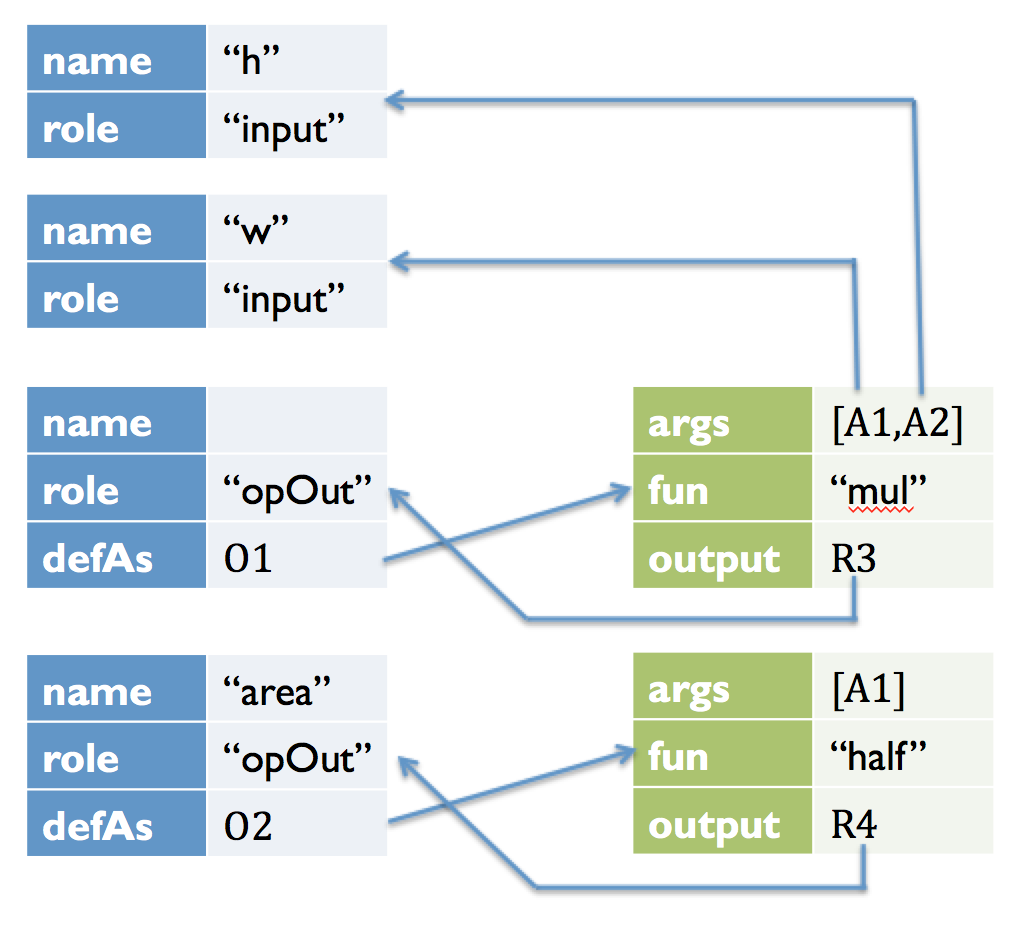
\includegraphics[width=0.6\textwidth]{./memory-layout.png}
\begin{small}
\begin{verbatim} 
class XManFunctions(object):
    @staticmethod
    def input(default=None):
        return Register(role='input',default=default)
    ...
    @staticmethod
    def mul(a,b):
        return XManFunctions.registerDefinedByOperator('mul',a,b)
    ...
    @staticmethod
    def registerDefinedByOperator(fun,*args):
        reg = Register(role='operationOutput')
        op = Operation(fun,*args)
        reg.definedAs = op
        op.outputReg = reg
        return reg
\end{verbatim} 
\end{small}
\end{center}
\label{fig:memory}
\caption{The Python data structures created by the \cd{Triangle}
  class.  Blue objects are \cd{Registers}, and green ones are
  \cd{Operations}.  Arrows are pointers.}
\end{figure}

The base \cd{XManFunctions} class defines a method \cd{input()} which
creates a register object that is marked as an ``input'', meaning that
it has no definition. (A similar method \cd{param()} creates a
register object that is marked as a ``parameter'', which like an input
has no definition.)  It also defines a few functions that correspond
to operators, like \cd{mul} and \cd{add}.  These return a register
object that is cross-linked to an \cd{Operation} object, as
illustrated in Figure~\ref{fig:memory}.  (The \cd{Register} class also
uses Python's operator overloading to so that syntax like \cd{h*w} is
  expanded to \cd{XManFunctions.mul(h,w)}.)

To produce the Wengert list, the \cd{setup()} command uses Python
introspection methods to add names to each register, based on the
Python variable that points to it, and generates new variable names
for any reachable registers that cannot be named with Python
variables.  Finally, the \cd{operationSequence} does a pre-order
traversal of the data structure to create a Wengert list.

\section{Assignment}

\wc{more hints: return delta[z]*d, to you can do the matrix-vector
  thing; sometimes output is used in derivatives.}

In this assignment you will use the automatic differentiation system described above
to implement two neural network architectures for character level entity classification. You 
will use \texttt{python} and \texttt{numpy} for this assigment.
The architectures you will implement are:
\begin{itemize}
    \item A three-layer feedforward network or Multilayer Perceptron (MLP)
    \item A Long Short Term Memory (LSTM) network followed by a feedforward network
\end{itemize}

Character level entity classification refers to determining the type of an entity 
given the characters which appear in its name as features. For example, given the name
``\cd{Noahshire}" you might guess that it is a \cd{Location}, and given the name
``\cd{Grebulons}"\footnote{\url{https://en.wikipedia.org/wiki/List_of_races_and_species_in_The_Hitchhiker\%27s_Guide_to_the_Galaxy#Grebulons}} you might guess that it is a \cd{Species}. 
Both of these are not real entities but highlight the possibility of using characters to classify entity types.

\section{Neural Networks}
\subsection{Mutlilayer Perceptron}
MLPs are the simplest neural network architecture consisting of multiple layers, each of 
which apply a linear transformation followed by non-linear mapping to their inputs:
\begin{align*}
    o_i &= f(\sum_{j=1}^{d_{in}} w_{ij} x_j + b_i) \\
            &= f(\mathbf{x}^T \mathbf{w_i} + b_i)
\end{align*}
Here $\mathbf{x} \in \mathbb{R}^{d_{in}}$ is the layer input and $o_i \in \mathbb{R}$ is the 
$i$-th output of the layer. $\mathbf{w_i}$, $b_i$ are layer parameters which we will optimize
during learning. The number of outputs at each layer is called the \textit{dimension}
of that layer and we denote it by $d_{out}$. We would like to use vector/matrix multiplications 
wherever possible to utilize their fast implementation in \texttt{numpy}, and combine the above
for all $i$ as:
\begin{equation*}
    \mathbf{o} = f(\mathbf{x}^T W + \mathbf{b})^T
\end{equation*}
$W=[w_1,w_2,\ldots,w_{d_{out}}] \in \mathbb{R}^{d_{in} \times d_{out}}$ stacks all the weight vectors 
horizontally, and $\mathbf{b} \in \mathbb{R}^{d_{out}}$ holds all the biases. The non-linearity $f$ is
applied elementwise.

To further speed-up the computation we can process a minibatch of inputs together. Let $X \in \mathbb{R}^{d_{in} \times N}$
be a matrix holding $N$ examples column-wise. We can compute the layer outputs for all of these together:
\begin{equation}
    O = f(X^T W + B)^T
\end{equation}
$B = \mathbf{1} \otimes \mathbf{b}^T \in \mathbb{R}^{N \times d_{out}}$ is a ``broadcasted" version of the bias
of appropriate dimensions. For this assigment you will use \cd{numpy} for all matrix operations, which takes care
of broadcasting automatically (see here\footnote{\url{https://docs.scipy.org/doc/numpy/user/basics.broadcasting.html}}
for details), hence we can use the vector $\mathbf{b}$ directly:
\begin{verbatim}
import numpy as np
Y = np.dot(X.transpose(), W) + b
O = elemwise_nonlinear_func(Y).transpose()
\end{verbatim}

In this assigment the nonlinearity we will use is the \texttt{Rectified Linear Unit (ReLU)}:
\begin{equation*}
    f(x) = 
    \begin{cases}
        x &\quad x>0 \\
        0 &\quad x\leq0
    \end{cases}
\end{equation*}
For vectors the nonlinearity is applied element-wise, and we can again use numpy broadcasting for
this:
\begin{verbatim}
def relu(X):
    return np.maximum(0,X) # X can be arbitrary shape
\end{verbatim}

We can set the size of the last layer of the MLP to produce a vector the same size as the number of
labels $L$ in our dataset. The operations described thus far map inputs to positive reals, but for 
classification tasks we are interested 
in obtaining a \textit{distribution} over class labels. This is usually done by
passing the output of MLP through a \texttt{softmax} layer:
\begin{equation}
    \label{eq:softmax}
    p_j = \frac{e^{o_j}}{\sum_{j'=1}^L e^{o_{j'}}}
\end{equation}
Note that $\mathbf{p}$ defines a valid distribution, and elements of $\mathbf{o}$ which have a
high relative value will have a high probability in $\mathbf{p}$. The above equation computes
$\mathbf{p}$ for a single $\mathbf{o}$, but in your code you should use \texttt{numpy}
operations to compute a minibatch of distributions $P$ from a minibatch of outputs $O$.

Lastly, we need to define a loss function which measures how far the distributions $P$ output from our network are from 
the target distributions $T$. We will use the cross-entropy loss for this:
\begin{equation}
    \label{eq:xentropy}
    J = - \frac{1}{N} \sum_{i=1}^N \sum_{j=1}^L T_{ij} \log P_{ij}
\end{equation}
Now we can take gradients of $J$ wrt to the parameters of the network and perform
Stochastic Gradient Descent (SGD).

To summarize, the first architecture you will implement for this assignment consists of an MLP
with one hidden layer, followed by a softmax layer \ref{eq:softmax} and cross-entropy loss 
\ref{eq:xentropy}.
Given an input $X$ and their associated targets $T$, the output is computed as:
\begin{align*}
    O^1 &= \text{relu}(X^T W^1 + \mathbf{b}^1) \\
    Y &= \text{relu}({O^1}^T W^2 + \mathbf{b}^2) \\
    P &= \text{softmax}(Y) \\
    J &= \text{cross-entropy}(T,P)
\end{align*}

\subsection{Long Short Term Memory}
The MLP is a powerful model -- with enough hidden units it can approximate any output, but it is not the most appropriate
model when the input is a sequence. For sequences, the input size of the MLP and consequently size of $W^1$, will
increase linearly with the size of the length of the sequence and might get prohibitively large. Instead, we would 
like to have a model which can loop over the input sequence, and starting from an initial state iteratively 
updates this state based on the input at that time step. LSTMs are one example of such a model
\footnote{An excellent introduction to LSTMs can be found at \url{http://colah.github.io/posts/2015-08-Understanding-LSTMs/}}.

Lets say we have a sequence of inputs $x_1,x_2,\ldots,x_M \in \mathbb{R}^{d_{in}}$, an initial \textit{cell state} $c_0 \in \mathbb{R}^{d_{out}}$ and an initial \textit{output}
$h_0 \in \mathbb{R}^{d_{out}}$. At time $t$ the LSTM does the following updates:
\begin{align*}
    i_t &= \sigma(x_t^T W_{i} + h_{t-1}^T U_{i} + b_{i})\\
    f_t &= \sigma(x_t^T W_{f} + h_{t-1}^T U_{f} + b_{f})\\
    o_t &= \sigma(x_t^T W_{o} + h_{t-1}^T U_{o} + b_{o})\\
    \tilde{c}_t &= tanh(x_t^T W_{c} + h_{t-1}^T U_{c} + b_{c})\\
    c_t &= f_t \odot c_{t-1} + i_t \odot \tilde{c}_t\\
    h_t &= o_t \odot tanh(c_t)
\end{align*}
Here $W_* \in \mathbb{R}^{d_{in} \times d_{out}}$, $U_* \in \mathbb{R}^{d_{out} \times d_{out}}$, $b_* \in \mathbb{R}^{d_{out}}$ 
are parameters, $\odot$ is an element-wise product and $\sigma$ is the sigmoid function:
\begin{equation}
    \sigma(x) = \frac{1}{1+ e^{-x}}
\end{equation}
Suppose we have a function \texttt{\_step} which takes $x_t$, $h_{t-1}$, $c_{t-1}$ and all the parameters
$W_*$, $U_*$, $B_*$ as input and returns $h_t$, $c_t$
 then the LSTM can be implemented as:
\begin{verbatim}
import numpy as np
def LSTM(x, params):
    h = np.zeros(d_out)
    c = np.zeros(d_out)
    for t=[1,2,...M]:
        h, c = _step(x[:,t], h, c, params)
    return h
\end{verbatim}
Where we assume \texttt{x} has the shape $d_{in} \times M$, i.e. each column holds the input for a particular $t$.
\textbf{Note:} The above equations are shown for single inputs $x$ for clarity. In your implementation you must use
minibatches $X$ of $N$ examples at a time, the same way as we did for the MLP. This would amount 

Now we are ready to implement the second architecture for this assignment. We will replace the hidden layer for MLP
in the previous section with an LSTM layer. hence the computation would be as follows:
\begin{align*}
    O^1 &= \text{LSTM}(X, \text{params}) \\
    Y &= \text{relu}({O^1}^T W^2 + \mathbf{b}^2) \\
    P &= \text{softmax}(Y) \\
    J &= \text{cross-entropy}(T,P)
\end{align*}
Where \texttt{params} is an object (python dictionary, for example) containing all the LSTM parameters.

\section{Data}

\section{Deliverables}

\section{Marking breakdown}

\end{document}

